\subsubsection{Templates}
\label{sec:3_WC_Templates}

Das folgende Kapitel basiert ausschließlich auf der Spezifikation von Templates des W3C \citereset \autocite{Weinstein.2013} und auf dem Artikel \glqq HTML's new Template Tag\grqq\ \citereset \autocite{BidelmanTemplate.2013}.

Laut W3C sind Templates autocite
\begin{quote}
\glqq
  a method for declaring inert DOM subtress in HTML and manipulating them to instantiate document fragments with identical contents.
\grqq
\end{quote}
Somit sind Templates eine Methode um inaktive DOM-Subtrees im HTML zu deklarieren und manipulieren, um so sämtliche identische Dokumentfragmente mit identischem Inhalt zu instanziieren.\\
In Web-Applikationen muss man oft den gleichen Subtree von Elementen öfters benutzen, mit den passenden Inhalt füllen und es zum Maintree hinzufügen. Man hat zum Beispiel eine Liste von Artikel, die man mit mehreren \lstinline|<li>| -Tags in das Dokument einfügen will. Des Weiteren kann jeder \lstinline|<li>|-Tag weitere Elemente, wie beispielsweise einen Link, ein Bild, einen Paragraphen, etc., enthalten. Bis jetzt bot HTML keine native Möglichkeit an, eine solche Aufgabenstellung zu lösen. Mehrere Beispiele, wie Entwickler diese Aufgabe lösten, sind:
\begin{enumerate}
\litem{Versteckte Elemente}
Dies galt unter den Entwicklern als die einfachste, aber auch als die ineffizienteste Methode. Man gab sein Markup irgendwo in das DOM (meist mit der CSS-Eigenschaft \lstinline|display: none;| am Parent-Element des Markups) und wann immer es gebraucht wurde, wurde es geklont, mit diversen Daten gefüllt und schlussendlich in das DOM eingefügt. Dies beinhaltet diverse Nachteile. Sämtliche Ressourcen, die im Markup verwendet wurden, sind bei Seitenaufruf geladen worden. Die Gesamtperformanz des Browsers wurde durch die vielzählige DOM-Traversierung beeinträchtigt.
\litem{String-Templates}
Man versuchte die Probleme der Methode mit \glqq versteckten Elementen\grqq\ zu beseitigen, indem man in einem \lstinline|<script>|-Tag ein Template mit einem String definiert. Dadurch, dass diese Methode hinsichtlich Laufzeit-Parsen von \lstinline|innerHtml| geht, können XSS-Attacks ermöglicht werden \todo{Information von: http://ejohn.org/blog/javascript-micro-templating}. Folglich wird ein Beispiel gezeigt, wo ein Template mit Hilfe eines Strings in einem \lstinline|<script>|-Tag definiert wird:
\begin{lstlisting}[language=HTML, caption=String-Template]
  <script type="text/html" id="test_Showcase">
  </script>
\end{lstlisting}
\end{enumerate}
Folgend wird an Hand eines Beispiels, wo eine Liste von Autos benutzt wird, der neue Standard zu Templates erläutert werden:\\

\begin{lstlisting}[language=HTML, caption={Web-Components Template-Standard}, label={lst:3_Templates}, escapeinside={@}{@}]
<template id="carTemplate">
  <li>
    <span class="carBrand"></span>
    <span class="carName"></span>
  </li>
</template>
\end{lstlisting}

Ein Template, wie das aus dem Code-Beispiel \ref{lst:3_Templates} auf Seite \pageref{lst:3_Templates}, kann sowohl im \lstinline|<head>|- als auch im \lstinline|<body>|-Tag definiert werden. Das Template, inklusive Subtree, ist inaktiv. Dies bedeutet, dass wenn sich ein \lstinline|<img>|-Tag mit einer validen Quelle in diesem Template befinden würde, würde der Browser dieses Bild nicht laden. Des Weiteren ist es nicht möglich via JavaScript ein Element des Templates zu selektieren.
\begin{lstlisting}[language=JavaScript, caption={Beispiel-Selektor eines Elements in einem Template, das nicht aktiven DOM ist}, label={lst:3_Selector_Example}]
  document.querySelectorAll('.carBrand').length; // length ist 0
\end{lstlisting}

\begin{figure}[h]
\centering
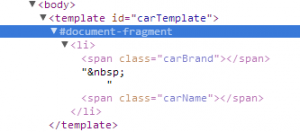
\includegraphics[height=3.0cm]{images/document_fragment.png}
\caption[
Visualisierung des DOM eines inaktiven Templates, Urldate: 04.2014
\newline
\small\texttt{\url{http://www.prevent-default.com/wp-content/uploads/2013/04/document-fragment-300x132.png}}
]{Visualisierung des DOM eines inaktiven Templates}
\label{fig:3_inactive_Template_DOM}
\end{figure}

In Abbildung \ref{fig:3_inactive_Template_DOM} auf Seite \pageref{fig:3_inactive_Template_DOM} wird gezeigt, dass das Template ein Dokument-Fragment ist. Dies bedeutet dass es ein eigenständiges Dokument ist und unabhängig vom ursprünglichen Dokument existiert. Folglich bedeutet dies, dass sämtliche \lstinline|<script>, <form>, <img>|-Tags etc. nicht verwendet werden.

\begin{lstlisting}[language=JavaScript, caption={Verwendung des Templates \ref{lst:3_Templates} auf Seite \pageref{lst:3_Templates}}, label={lst:3_Templates_Verwendung}, escapeinside={@}{@}]
@\label{lst:3_Templates_Verwendung_1}@var template = document.getElementById('carTemplate');
template.content.querySelector(".carBrand").length; // length ist 1

@\label{lst:3_Templates_Verwendung_2}@var car = template.content.cloneNode(true);
car.querySelector(".carBrand").innerHTML = "Seat";
car.querySelector(".carName").innerHTML = "Ibiza";

@\label{lst:3_Templates_Verwendung_3}@document.getElementById("carList").appendChild(car);
\end{lstlisting}
Code-Beispiel \ref{lst:3_Templates_Verwendung} auf Seite \pageref{lst:3_Templates_Verwendung} basiert auf dem in Code-Beispiel \ref{lst:3_Templates} auf Seite \pageref{lst:3_Templates} definierten Template. Zuerst wird sich in Zeile \ref{lst:3_Templates_Verwendung_1} des Code-Beispiels \ref{lst:3_Templates_Verwendung} das vorher definierte Template in die Variable \lstinline|template| geholt. Daraufhin wird der gesamte Knoten in Zeile \ref{lst:3_Templates_Verwendung_2} mit Hilfe einer \lstinline|deep-copy| geklont und des Weiteren mit Daten befüllt. Damit das mit Daten befüllte Listenelement auch sichtbar wird, wird es in Zeile \ref{lst:3_Templates_Verwendung_3} in das aktive DOM eingefügt.
